\section{Introduction}
\label{sec:intro}

The problem of fairly allocating items among multiple agents has garnered significant attention in the fields of
computer science, multi-agent systems, and game theory.
It finds applications in many real-world scenarios such as dividing inheritance, dividing natural resources among countries or states, allocating public housing, divorce settlements, and distributing research papers to reviewers.
%One of the oldest-known applications occurs in the Bible \cite{bible_cut_and_choose}.

Research in fair division began with the study of \emph{divisible} resources (e.g., land, water, cake)
\cite{steinhaus1940sur,stromquist1980how,varian1974equity}.
\emph{Fairness} was formally defined in two different ways:
\emph{envy-freeness} (EF) and \emph{proportionality} (PROP).
EF means that each agent believes that she got the best bundle of items compared to others,
and PROP means that each agent's value for her own bundle is at least a $1/n$ fraction
of her value of the entire set of items, where $n$ is the number of agents.
By the 1980s, EF and PROP allocations were shown to exist,
and algorithms for finding such allocations were given
\cite{steinhaus1940sur,stromquist1980how,varian1974equity}.

These positive results break down when the items become indivisible.
For example, when 5 identical goods must be divided among two agents,
an EF or PROP allocation cannot exist.
However, one can still aim for \emph{approximate} fairness;
an allocation that gives 3 goods to one agent and 2 goods to the other
is intuitively as fair as possible.
But when we move away from this simple example to the general setting where
items are not identical and agents have heterogeneous preferences,
formally defining (approximate) fairness becomes challenging.
Consequently, many definitions of fairness have been proposed for the indivisible setting.

EF was relaxed to a notion called \emph{EF1}\fairDefLater{} (envy-freeness up to one item),
and algorithms guaranteeing EF1 allocations were given \cite{budish2011combinatorial,lipton2004approximately}.
However, EF1 was considered a somewhat weak fairness notion,
%\footnote{Consider dividing a house and two cars among two agents.
%Intuitively, the agent who gets the house shouldn't get anything else,
%but allocating the house and a car to one agent and only a car to the other is EF1.},
so a stronger notion called \emph{EFX}\fairDefAgain{} (envy-freeness up to any item)
\cite{caragiannis2019unreasonable} was extensively studied.
Despite considerable effort from researchers, the existence of EFX allocations
remains an important open problem.
Hence, relaxations of EFX \cite{caragiannis2023new,amanatidis2020multiple,chaudhury2021little}
and the existence of EFX in special cases \cite{chaudhury2024efx,plaut2020almost,amanatidis2021maximum}
have been studied.
%
A similar story played out for relaxations of PROP:
The existence of PROP1\fairDefAgain{} (proportional up to one item) was easy to prove \cite{aziz2021fair},
but stronger notions like MMS\fairDefAgain{} (maximin share) \cite{kurokawa2018fair}
and PROPx\fairDefAgain{} (proportional up to any item) \cite{aziz2020polynomial}
were shown to be infeasible, so their relaxations have been studied
\cite{kurokawa2018fair,akrami2024breaking,baklanov2021propm,caragiannis2023new,kobayashi2025proportional}.
Moreover, insisting on polynomial-time computability,
compatibility with notions of efficiency (like Pareto optimality),
or other constraints \cite{gourves2014near,bouveret2017fair,biswas2018fair,equbal2024fair}
makes the problem harder, necessitating the use of even weaker fairness notions.

Hence, for the problem of fairly allocating indivisible items,
several notions of fairness have been proposed,
occupying varying levels of perceived fairness.
We believe a systematic study of the relative merits of different fairness notions
is key to informing practical applications and further research in this area.
We contribute towards this objective by doing a
comprehensive comparison of 22 different fairness notions
through the lens of \emph{implications}.

Formally, a fairness notion $F_1$ \emph{implies} another notion $F_2$
if every $F_1$-fair allocation is also $F_2$-fair.
On the other hand, if we can find an $F_1$-fair allocation that is not $F_2$-fair,
we get a \emph{counterexample}, i.e., a proof that $F_1$ does not imply $F_2$.
For additive valuations, which is the most-studied setting in fair allocation,
we give a near-complete picture of implications among fairness notions:
for almost every pair of notions, we either prove that
one notion implies the other, or we give a counterexample.
These results put fairness notions into a hierarchy,
and the counterexamples shed light on the pros and cons of different notions.
See \cref{fig:additive-nny} for the implications we show for additive goods and additive chores,
and \cref{sec:dags} for similar figures for other fair division settings.

\begin{figure*}[!htb]
\centering
\begin{subfigure}{0.45\textwidth}
    \centering
    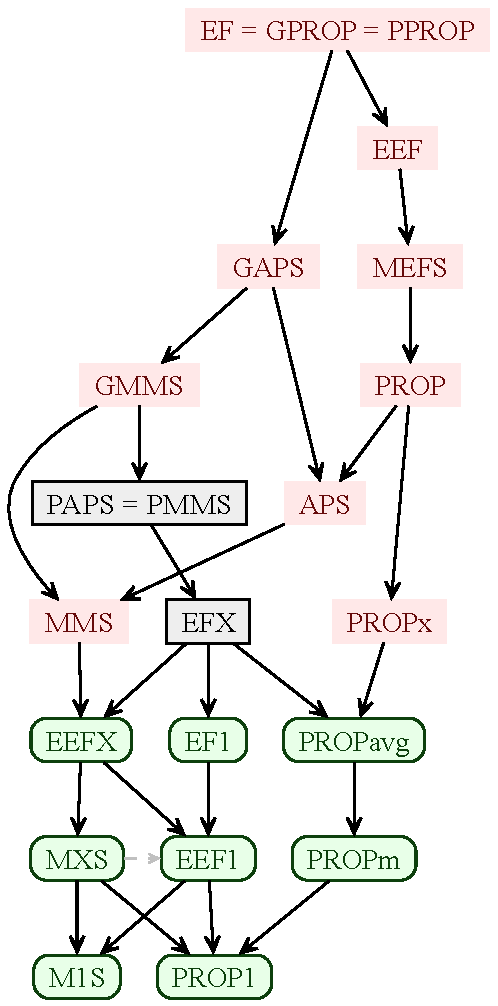
\includegraphics[scale=0.6]{dags/additive-nonneg-nny.pdf}
    \caption{Goods}
\end{subfigure}
\hfill
\begin{subfigure}{0.5\textwidth}
    \centering
    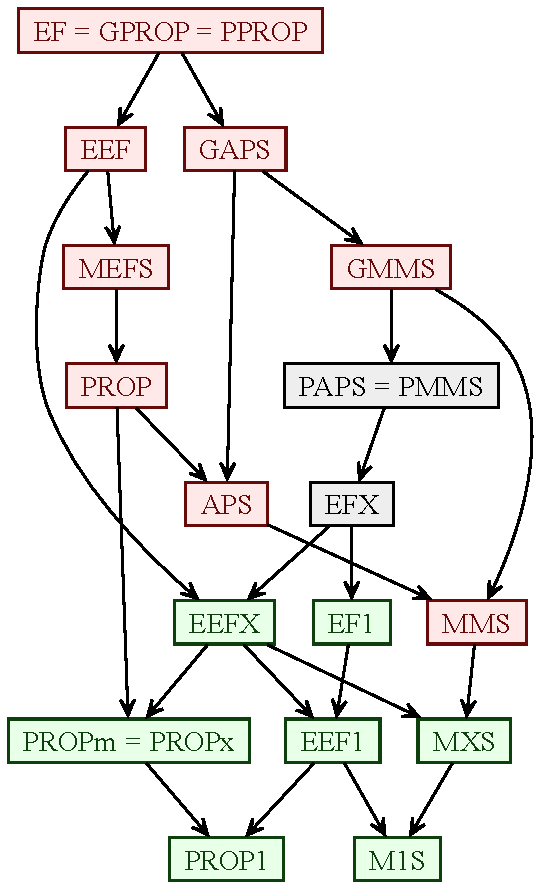
\includegraphics[scale=0.6]{dags/additive-nonpos-nny.pdf}
    \caption{Chores}
\end{subfigure}
\caption[Additive goods and chores with equal entitlements]{%
Implications between fairness notions for additive valuations over goods and over chores
when agents have equal entitlements. There is a vertex for each fairness notion.
Notion $F_1$ implies notion $F_2$ iff there is a path from $F_1$ to $F_2$ in the graph
(except that it is not known whether MXS implies EEF1 for goods).
Borderless vertices (red) are infeasible notions,
vertices with rounded corners (green) are feasible notions,
and the feasibility of the remaining vertices (gray) are open problems.
Note that goods and chores have some key differences, e.g.,
for goods, PROP $\fimplies$ MMS $\fimplies$ EEF1 $\fimplies$ PROP1,
but for chores, MMS $\nfimplies$ PROP1, and PROP $\nfimplies$ EEF1.}
\label{fig:additive-nny}
\end{figure*}

Many different settings of fair division have been considered in the literature:
goods vs chores vs mixed manna, equal vs unequal entitlements, and different classes of valuation functions.
Special cases have also been studied, like identical valuations or fair division among just two agents.
Although our primary focus is equal entitlements and additive valuations over goods and over chores,
we also consider all the other settings, i.e., all combinations of the above aspects of fair division.
At first, this leads to a combinatorial explosion of different settings.
However, we get around this by encoding our implication and non-implication results in a machine-readable format
and implementing an \emph{inference engine} that uses these results to automatically deduce new results.

For example, if we ask the inference engine
``Does epistemic envy-freeness (EEF\fairDefAgain{}) imply maximin share (MMS) for goods with additive valuations?",
it would give an affirmative answer based on these three results we show in the paper:
\begin{enumerate}
\item EEF implies minimum-EF-share fairness (MEFS\fairDefAgain{}).
\item MEFS implies PROP under subadditive valuations
    (\cref{thm:impl:mefs-to-prop} in \cref{sec:impls-extra}).
\item PROP implies MMS for superadditive valuations
    (\cref{thm:impl:prop-to-wmms} in \cref{sec:impls-extra}).
\end{enumerate}

\subsection{Our Contributions}

%\begin{enumerate}
We prove several implications and counterexamples between fairness notions for various settings.
The implications put the notions into a hierarchy,
and the counterexamples illustrate the relative merits of different fairness notions.
For the most important setting of equal entitlements and additive valuations,
we give a near-complete picture of implications for goods, chores, and mixed manna.

We wrote a computer program, called an \emph{inference engine}, to automate part of our work.
After proving some (non-)implications manually (\cref{sec:summary}),
we fed those results into the inference engine,
which then generated many more (non-)implications (\cref{fig:additive-nny,sec:dags}).
We implement our inference engine as a web application in JavaScript%
\ifx\version\versionDefault
\ (\url{https://sharmaeklavya2.github.io/cpigjs/fairDiv/})%
\fi.
The engine can be extended beyond fair division (\cref{sec:cpig}),
and so may be of independent interest.

Many of the implications we prove in \cref{sec:summary} were already known
for additive valuations and equal entitlements; we extended them to more general settings.
On the other hand, most of the counterexamples in \cref{sec:summary} are new.
We give the simplest possible counterexamples to make the distinctions
between fairness notions as clear and accessible as possible.
%While the examples may appear straightforward, discovering them was non-trivial,
%especially given the large number needed to provide a complete picture of implications.

Some fairness notions were originally defined only for very specific fair division settings.
E.g., EFX was defined in \cite{caragiannis2019unreasonable} for additive goods.
%(Although EFX was also defined for mixed manna by many subsequent works,
%there are now several competing definitions, and their relative merits are unclear.)
We extend all fairness notions to the most general fair division setting we consider:
mixed manna with unequal entitlements.
In some cases, picking an appropriate definition was non-trivial,
and we present several observations to motivate the definitions we propose.
%\end{enumerate}

\subsection{Related Work}
\label{sec:intro:related-work}

\cite{amanatidis2023fair} give a survey on recent progress and open problems in fair division,
where they consider many different fair division settings and fairness notions.

The most common setting in fair division is equally-entitled agents
having additive valuations over goods. For this setting, \cite{bouveret2016characterizing}
studied implications among 5 fairness notions: CEEI, EF, PROP, MMS, and min-max-share
(also called minimum EF share).
\cite{amanatidis2018comparing} studies implications between
multiplicative approximations of fairness notions.
\cite{aziz2021fair} consider implications between EF, PROP, EF1, and PROP1 for mixed manna instead.
\cite{chakraborty2024weighted} studies implications for the weighted setting
among EF1, PROP1, APS, MNW, and other notions.
Over time, as new fairness notions were proposed
\cite{caragiannis2023new,babaioff2023fair,barman2018groupwise,aziz2018knowledge},
their connections with other well-established notions were studied.
However, the above works only consider a limited number of fairness notions and fair division settings.
Our work, on the other hand, aims to be more exhaustive, and thus, have broader applicability.

\subsection{Structure of the Paper}

In \cref{sec:prelims}, we formally define the fair division problem, describe different fair division settings, and introduce associated notation.
In \cref{sec:notions}, we describe the fairness notions that we consider.
In \cref{sec:summary}, we present a summary of our results, i.e.,
a list of implications and counterexamples between pairs of fairness notions.
In \cref{sec:cpig}, we describe our inference engine.
\Cref{sec:conclusion} contains concluding remarks and open problems.

\ifx\version\versionDefault\else
Due to space constraints, we move several details to appendices,
which can be found in the full version of the paper included in the supplementary material.
\fi
\Cref{sec:settings-extra,sec:notions-extra} contain details on fair division settings and fairness notions.
\Cref{sec:impls-extra,sec:cex-extra} contain proofs of our (non-)implication results.
\Cref{sec:feas} contains results on (in)feasibility of fairness notions.
\Cref{sec:dags} contains several implication diagrams, i.e.,
analogues of \cref{fig:additive-nny} for other fair division settings.
